% Pricing defects in evaluation environments by expected loss.
%
% No result-derived number is typed in this file. Each is a macro from
% generated/numbers.tex, written by scripts/export_paper_tables.py from the
% committed results/*.json; tables and figures come from the same script.
% tests/test_paper.py fails if a digit appears in the prose outside a short
% allow-list, if generated/ is stale, or if the built PDF loses a number.
\documentclass[11pt]{article}
\usepackage[margin=1in]{geometry}
\usepackage[T1]{fontenc}
\usepackage{lmodern}
\usepackage{amsmath,amssymb}
\usepackage{booktabs}
\usepackage{tikz}
\usepackage{pgfplots}
\pgfplotsset{compat=1.17}
\usepackage[numbers,sort&compress]{natbib}
\usepackage[hidelinks]{hyperref}
\usepackage[font=footnotesize,skip=3pt]{caption}
\usepackage{microtype}
\sloppy
\makeatletter
\renewcommand\paragraph{\@startsection{paragraph}{4}{\z@}%
  {1.6ex \@plus .4ex \@minus .2ex}{-1em}{\normalfont\normalsize\bfseries}}
\makeatother
\setlength{\tabcolsep}{4pt}
\setlength{\textfloatsep}{8pt plus 2pt minus 2pt}
\setlength{\floatsep}{8pt plus 2pt minus 2pt}

% GENERATED by scripts/export_paper_tables.py from results/*.json. Do not edit.
% Every result-derived number in paper/assay.tex is one of these macros.
\newcommand{\ablClaudeSec}{261.7}
\newcommand{\ablQwenAttempts}{10}
\newcommand{\ablQwenSec}{97.0}
\newcommand{\ablScriptedThenSec}{2.2}
\newcommand{\agDetLossThen}{240.0}
\newcommand{\agK}{4}
\newcommand{\agMissEnvs}{3}
\newcommand{\agSlice}{5}
\newcommand{\assayAbsentFA}{0}
\newcommand{\assayCleanFA}{14}
\newcommand{\assayDirtyFA}{3}
\newcommand{\assayMissCost}{40.0}
\newcommand{\bootSeed}{11}
\newcommand{\chHits}{3}
\newcommand{\chK}{4}
\newcommand{\costCeilHi}{849.5}
\newcommand{\costCeilLo}{141.6}
\newcommand{\costEngHi}{250}
\newcommand{\costEngLo}{75}
\newcommand{\costFloorHi}{4.43}
\newcommand{\costFloorLo}{0.04}
\newcommand{\costGpuHi}{720}
\newcommand{\costGpuLo}{24}
\newcommand{\costMinHi}{30}
\newcommand{\costMinLo}{5}
\newcommand{\costSamples}{1{,}699}
\newcommand{\costSpot}{0.46}
\newcommand{\critCross}{1371}
\newcommand{\critCrossRatio}{11.4}
\newcommand{\critErrPct}{1042}
\newcommand{\critShipped}{120}
\newcommand{\extBenchAssay}{640.0}
\newcommand{\extBenchFloor}{968.0}
\newcommand{\extCross}{348}
\newcommand{\extFlatAssay}{6.0}
\newcommand{\extFlatFloor}{121.0}
\newcommand{\extHiSaved}{121}
\newcommand{\extLoSaved}{\ensuremath{-}4}
\newcommand{\extLossAssay}{45.0}
\newcommand{\extLossAuditor}{44.0}
\newcommand{\extLossCheckEnv}{320.0}
\newcommand{\extLossFloor}{121.0}
\newcommand{\extLossNothing}{328.0}
\newcommand{\extMiss}{1}
\newcommand{\extPrec}{0.545}
\newcommand{\extProdAssay}{250.0}
\newcommand{\extProdDelta}{8.0}
\newcommand{\extProdFloor}{242.0}
\newcommand{\extRec}{0.857}
\newcommand{\extSaved}{76.0}
\newcommand{\extSpur}{5}
\newcommand{\floorAbsent}{132}
\newcommand{\floorClean}{108}
\newcommand{\floorDirty}{234}
\newcommand{\floorPerEnvClean}{16}
\newcommand{\floorRestricted}{342}
\newcommand{\foFalse}{0}
\newcommand{\foTrials}{50}
\newcommand{\foUpper}{5.8}
\newcommand{\fofDetected}{10}
\newcommand{\fofPos}{12}
\newcommand{\fofTasks}{102}
\newcommand{\fofThreshold}{59}
\newcommand{\gateBadRuns}{1}
\newcommand{\gateBestLoss}{43.0}
\newcommand{\gateDetLoss}{57.0}
\newcommand{\gateGoodMax}{14.0}
\newcommand{\gateGoodMin}{13.0}
\newcommand{\gateGoodRuns}{6}
\newcommand{\gateMaxSaved}{14.0}
\newcommand{\gateMeanSaved}{2.4}
\newcommand{\gateMedianSaved}{14.0}
\newcommand{\gateRunValues}{14.0, \ensuremath{-}65.0, 14.0, 14.0, 13.0, 14.0, 13.0}
\newcommand{\gateRuns}{7}
\newcommand{\gateWorstLoss}{122.0}
\newcommand{\gateWorstSaved}{65.0}
\newcommand{\grpoPct}{20}
\newcommand{\grpoRows}{60}
\newcommand{\grpoTotalRows}{300}
\newcommand{\hiLossAgentTools}{3883}
\newcommand{\hiLossAlwaysModal}{2909}
\newcommand{\hiLossAssay}{142}
\newcommand{\hiLossAssayAuditor}{126}
\newcommand{\hiLossCheckEnv}{4552}
\newcommand{\hiLossDirectPrompt}{3366}
\newcommand{\hiLossFlagEverything}{492}
\newcommand{\hiLossFlagNothing}{4560}
\newcommand{\hiLossStratRandom}{4071}
\newcommand{\hiSavedAgentTools}{3838}
\newcommand{\hiSavedAlwaysModal}{2865}
\newcommand{\hiSavedCheckEnv}{4499}
\newcommand{\hiSavedCheckEnvVsNothing}{40}
\newcommand{\hiSavedDPvsRandom}{1060}
\newcommand{\hiSavedDirectPrompt}{3328}
\newcommand{\hiSavedFlagEverything}{471}
\newcommand{\hiSavedFlagNothing}{4510}
\newcommand{\hiSavedRandomVsAT}{343}
\newcommand{\hiSavedStratRandom}{4028}
\newcommand{\highCross}{457}
\newcommand{\kappaAgree}{85}
\newcommand{\kappaEnvs}{24}
\newcommand{\kappaVal}{0.278}
\newcommand{\loLossAgentTools}{1753}
\newcommand{\loLossAlwaysModal}{1315}
\newcommand{\loLossAssay}{8}
\newcommand{\loLossAssayAuditor}{1}
\newcommand{\loLossCheckEnv}{2056}
\newcommand{\loLossDirectPrompt}{1451}
\newcommand{\loLossFlagEverything}{453}
\newcommand{\loLossFlagNothing}{2080}
\newcommand{\loLossStratRandom}{1767}
\newcommand{\loSavedAgentTools}{1681}
\newcommand{\loSavedAlwaysModal}{1248}
\newcommand{\loSavedCheckEnv}{1979}
\newcommand{\loSavedCheckEnvVsNothing}{0}
\newcommand{\loSavedDPvsRandom}{\ensuremath{-}61}
\newcommand{\loSavedDirectPrompt}{1388}
\newcommand{\loSavedFlagEverything}{330}
\newcommand{\loSavedFlagNothing}{2001}
\newcommand{\loSavedRandomVsAT}{\ensuremath{-}486}
\newcommand{\loSavedStratRandom}{1692}
\newcommand{\lossAgentTools}{2746.0}
\newcommand{\lossAlwaysModal}{2055.0}
\newcommand{\lossAssay}{57.0}
\newcommand{\lossAssayAuditor}{44.0}
\newcommand{\lossCheckEnv}{3216.0}
\newcommand{\lossDirectPrompt}{2343.0}
\newcommand{\lossFlagEverything}{474.0}
\newcommand{\lossFlagNothing}{3232.0}
\newcommand{\lossGapLLMvsRandom}{495.0}
\newcommand{\lossStratRandom}{2838.0}
\newcommand{\missAgentTools}{41}
\newcommand{\missAlwaysModal}{44}
\newcommand{\missAssay}{0}
\newcommand{\missAssayAuditor}{1}
\newcommand{\missCheckEnv}{52}
\newcommand{\missDirectPrompt}{41}
\newcommand{\missFlagEverything}{0}
\newcommand{\missFlagNothing}{54}
\newcommand{\missStratRandom}{49}
\newcommand{\nAuthored}{15}
\newcommand{\nClasses}{16}
\newcommand{\nClassesAbsent}{4}
\newcommand{\nClassesPresent}{12}
\newcommand{\nCleanEnv}{9}
\newcommand{\nEnv}{33}
\newcommand{\nExtDerived}{3}
\newcommand{\nExtHand}{5}
\newcommand{\nExtPlanted}{7}
\newcommand{\nExternal}{8}
\newcommand{\nFixtures}{12}
\newcommand{\nPlanted}{54}
\newcommand{\nPlantedExtDerived}{5}
\newcommand{\nPlantedHand}{2}
\newcommand{\nPlantedHere}{47}
\newcommand{\nRedTeamFoundAfter}{10}
\newcommand{\nResamples}{10{,}000}
\newcommand{\nRetractions}{22}
\newcommand{\nSelfAuthored}{25}
\newcommand{\nSpurAssay}{17}
\newcommand{\nTP}{53}
\newcommand{\nThirdFormat}{10}
\newcommand{\nUnchecked}{1}
\newcommand{\noHarborN}{28}
\newcommand{\pctCheckEnvVsNothing}{0.50}
\newcommand{\pctFloorAbsent}{27.8}
\newcommand{\pctFloorClean}{22.8}
\newcommand{\precAgentTools}{0.277}
\newcommand{\precAlwaysModal}{0.303}
\newcommand{\precAssay}{0.757}
\newcommand{\precAssayAuditor}{0.930}
\newcommand{\precCheckEnv}{1.000}
\newcommand{\precDirectPrompt}{0.295}
\newcommand{\precFlagEverything}{0.102}
\newcommand{\precFlagNothing}{0.000}
\newcommand{\precStratRandom}{0.098}
\newcommand{\predGateSaving}{13.0}
\newcommand{\prodRatio}{480}
\newcommand{\profAssayBench}{736.0}
\newcommand{\profAssayFlat}{18.0}
\newcommand{\profAssayProd}{274.0}
\newcommand{\profAssayResearch}{57.0}
\newcommand{\profFloorBench}{3792.0}
\newcommand{\profFloorFlat}{474.0}
\newcommand{\profFloorProd}{948.0}
\newcommand{\profFloorResearch}{474.0}
\newcommand{\profHiSavedBench}{3768}
\newcommand{\profHiSavedFlat}{475}
\newcommand{\profHiSavedProd}{942}
\newcommand{\profHiSavedResearch}{471}
\newcommand{\profLoSavedBench}{1800}
\newcommand{\profLoSavedFlat}{435}
\newcommand{\profLoSavedProd}{180}
\newcommand{\profLoSavedResearch}{330}
\newcommand{\profSavedBench}{3056.0}
\newcommand{\profSavedFlat}{456.0}
\newcommand{\profSavedProd}{674.0}
\newcommand{\profSavedResearch}{417.0}
\newcommand{\realCheckDetected}{1}
\newcommand{\realCheckPlanted}{4}
\newcommand{\recAgentTools}{0.241}
\newcommand{\recAlwaysModal}{0.185}
\newcommand{\recAssay}{0.982}
\newcommand{\recAssayAuditor}{0.982}
\newcommand{\recCheckEnv}{0.037}
\newcommand{\recChecked}{1.000}
\newcommand{\recDirectPrompt}{0.241}
\newcommand{\recFlagEverything}{1.000}
\newcommand{\recFlagNothing}{0.000}
\newcommand{\recStratRandom}{0.093}
\newcommand{\rtBroken}{12}
\newcommand{\rtClaims}{21}
\newcommand{\rtPartial}{2}
\newcommand{\rtSurvives}{6}
\newcommand{\rtWeak}{1}
\newcommand{\sabDetected}{0}
\newcommand{\sabFindings}{0}
\newcommand{\sabGold}{12}
\newcommand{\savedAgentTools}{2689.0}
\newcommand{\savedAlwaysModal}{1998.0}
\newcommand{\savedCheckEnv}{3159.0}
\newcommand{\savedCheckEnvVsNothing}{16.0}
\newcommand{\savedDPvsRandom}{495.0}
\newcommand{\savedDirectPrompt}{2286.0}
\newcommand{\savedFlagEverything}{417.0}
\newcommand{\savedFlagNothing}{3175.0}
\newcommand{\savedRandomVsAT}{\ensuremath{-}92.0}
\newcommand{\savedRestricted}{285.0}
\newcommand{\savedStratRandom}{2781.0}
\newcommand{\scriptedAttempts}{6}
\newcommand{\scriptedSeconds}{3.8}
\newcommand{\selfLossAssay}{12.0}
\newcommand{\selfLossFloor}{353.0}
\newcommand{\selfN}{25}
\newcommand{\sepAgentTools}{separated}
\newcommand{\sepAlwaysModal}{separated}
\newcommand{\sepCheckEnv}{separated}
\newcommand{\sepDirectPrompt}{separated}
\newcommand{\sepFlagEverything}{separated}
\newcommand{\sepFlagNothing}{separated}
\newcommand{\sepStratRandom}{separated}
\newcommand{\sgFPPct}{3.3}
\newcommand{\sgFPRuns}{2}
\newcommand{\sgNNeg}{20}
\newcommand{\sgNPos}{5}
\newcommand{\sgNegRuns}{60}
\newcommand{\sgPosRuns}{15}
\newcommand{\sgTPRuns}{14}
\newcommand{\spurAgentTools}{34}
\newcommand{\spurAlwaysModal}{23}
\newcommand{\spurAssay}{17}
\newcommand{\spurAssayAuditor}{4}
\newcommand{\spurCheckEnv}{0}
\newcommand{\spurDirectPrompt}{31}
\newcommand{\spurFlagEverything}{474}
\newcommand{\spurFlagNothing}{0}
\newcommand{\spurStratRandom}{46}
\newcommand{\tauAllExpTP}{20.41}
\newcommand{\tauAllFlag}{54}
\newcommand{\tauAllP}{0.486}
\newcommand{\tauAllPrec}{0.389}
\newcommand{\tauAllRec}{0.339}
\newcommand{\tauAllTP}{21}
\newcommand{\tauBase}{0.378}
\newcommand{\tauDbPos}{5}
\newcommand{\tauEvalAmbDet}{5}
\newcommand{\tauEvalAmbPos}{21}
\newcommand{\tauFloorPrec}{0.378}
\newcommand{\tauNarExpTP}{8.70}
\newcommand{\tauNarFlag}{23}
\newcommand{\tauNarP}{0.040}
\newcommand{\tauNarPrec}{0.565}
\newcommand{\tauNarRec}{0.210}
\newcommand{\tauNarTP}{13}
\newcommand{\tauPos}{62}
\newcommand{\tauTasks}{164}
\newcommand{\tpfLossAssay}{0.0}
\newcommand{\tpfLossFloor}{132.0}
\newcommand{\tpfN}{10}

\newcommand{\assay}{\textsc{Assay}}
\newcommand{\fe}{\texttt{flag\_everything}}
\newcommand{\fp}{\texttt{flag\_present}}
\newcommand{\pf}{\texttt{prevalence\_floor}}

\title{Pricing Defects in Evaluation Environments by Expected Loss:\\
A Probe Battery Evaluated Against Trivial and Prevalence-Aware Floors}
\author{Caio Theodoro\\\small Avenza Labs (\texttt{avenza.cloud}) \and Jo\~{a}o Vitor Basso Sberse\\\small Avenza Labs (\texttt{avenza.cloud}) \and Matheus Theodoro\\\small Avenza Labs (\texttt{avenza.cloud})}
\date{First version 28 August 2026; this version 23 November 2026}

\begin{document}
\maketitle

\begin{abstract}
\noindent
Reinforcement-learning environments and evaluation suites are routinely deployed on the strength of
verifiers that are rarely checked mechanically. \assay{} is a deterministic-by-default battery of
eleven probe families covering \nClasses{} defect classes that executes an environment and prices
missed defects and false alarms on a single expected-loss scale under a stated cost profile.
On \nEnv{} environments carrying \nPlanted{} planted defects under the \texttt{research-run}
profile, \assay{} achieves an expected loss of \lossAssay{} (95\% CI \loLossAssay--\hiLossAssay{}),
saving \savedRestricted{} (\loSavedRestricted--\hiSavedRestricted{}, \sepRestricted{}) against the
restricted constant floor that flags only the \nClassesPresent{} occurring defect classes
(\floorRestricted{}) and \savedFlagEverything{} (\loSavedFlagEverything--\hiSavedFlagEverything{},
\sepFlagEverything{}) against the unrestricted \fe{} floor (\lossFlagEverything{}, CI
\loLossFlagEverything--\hiLossFlagEverything{}), separating against \fe{} on all four cost
profiles. Post hoc against an in-sample Bayes-optimal prevalence-aware constant floor
(\lossPrevResearch{}), \assay{} saves \savedPrevResearch{} (\loSavedPrevResearch--\hiSavedPrevResearch{},
separated on three of four cost profiles and not separated on \texttt{production-training}).
Precision is \precAssay{} (\nSpurAssay{} false alarms, \assayCleanFA{} on five environments with no
correct answer) and recall is \recAssay{} (\missAssay{} true misses, \nUnchecked{} unchecked defect
priced as a miss). Because \nSelfAuthored{} of \nEnv{} environments are author-constructed, the
\nExternal{} third-party environments form the external control: there the saving over \fe{} is
\extSaved{} (95\% CI \extLoSaved{} to \extHiSaved{}, not separated), and against \tauPos{} defects
an independent team confirmed in $\tau^2$-bench, full-battery recall is \tauAllRec{} ($p=\tauAllP$,
indistinguishable from random flagging). An opt-in language-model gate meant to withhold false
alarms on no-answer environments deleted two real defects in \gateBadRuns{} of \gateRuns{}
identical runs, reducing its mean saving over the deterministic battery to \gateMeanSaved{} (median
\gateMedianSaved{}). The code is Apache-2.0; deterministic arms reproduce without a GPU or API key.
\end{abstract}

\section{Introduction}
\label{sec:intro}

An RL environment or evaluation suite pairs a task with a verifier. When the verifier diverges from
the task, the failure is silent: a trained policy optimises the verifier instead of the intended
behaviour, and the flaw surfaces weeks later as an implausible reward curve or a benchmark that must
be repaired by hand. SWE-bench Verified required manual triage by 93 developers over 1,699
samples~\citep{openai2024verified}, and subsequent audits still uncovered plausible-but-wrong
patches that pass~\citep{wang2025solved} and solutions leaked in issue
text~\citep{aleithan2024swebenchplus}. WebArena was re-issued for a loose substring
evaluator~\citep{elhattami2025webarenaverified}. Across agent benchmarks more broadly, systematic
reviews have argued for cost-controlled, variance-aware evaluation~\citep{kapoor2024agents} and
explicit benchmark-quality standards~\citep{reuel2024betterbench}.

This paper evaluates \assay{}, an execution-based probe battery that checks environments before
training or reporting. Rather than claiming higher raw recall than existing auditors, \assay{}
frames environment auditing as cost-sensitive classification~\citep{elkan2001}: every missed defect
carries a severity-weighted failure cost, every false alarm carries an inspection cost, and both
are measured on one scale. That framing changes the decisive baseline. Beating an incumbent
interface linter proves little when the linter checks almost nothing; the baseline an auditor must
clear is an input-ignoring floor that achieves high or complete recall by construction---\fe{}, a
restricted floor over occurring defect classes, and a prevalence-aware Bayes-optimal constant
policy.

On a \nEnv{}-environment corpus under the \texttt{research-run} cost profile, \assay{} attains an
expected loss of \lossAssay{}, saving \savedRestricted{} (\loSavedRestricted--\hiSavedRestricted{})
over the restricted floor (\floorRestricted{}) and \savedPrevResearch{}
(\loSavedPrevResearch--\hiSavedPrevResearch{}) over a post hoc Bayes-optimal prevalence-aware floor
(\lossPrevResearch{}), while also revealing clearly where evidence stops: on the \nExternal{}
third-party environments the saving over \fe{} does not separate from zero, and on independently
labelled $\tau^2$-bench defects full-battery recall is at chance. Our contributions are:

\begin{itemize}\setlength\itemsep{1pt}\setlength\parskip{0pt}
\item \textbf{A cost-sensitive execution-based probe battery.} Eleven deterministic-by-default probe
families covering \nClasses{} defect classes across four ecosystems, with explicit
\texttt{NOT\_APPLICABLE} reporting and an expected-loss harness across four cost profiles
(\S\ref{sec:method}, Tables~\ref{tab:classes}--\ref{tab:costs}).
\item \textbf{Evaluation against unrestricted, restricted, and prevalence-aware floors.} A unified
comparison of nine arms alongside post hoc restricted and Bayes-optimal prevalence-aware constant
floors across all four cost profiles, plus exact sensitivity to the miss-cost constant
(\S\ref{sec:headline}--\ref{sec:cost}).
\item \textbf{External-scope and independent-label measurements.} Provenance-split scoring isolating
the \nExternal{} third-party environments, task-level recall against \tauPos{} independently
confirmed $\tau^2$-bench defects, and a third-party-scored evaluation on ScienceAgentBench
(\S\ref{sec:splits}--\ref{sec:external}).
\item \textbf{Empirical boundaries of an opt-in agent layer.} Repeated-run reliability of a semantic
LLM gate across \gateRuns{} identical runs and ablations comparing prompted, trained, and scripted
reward-hack challengers (\S\ref{sec:agent}).
\end{itemize}

\section{Related work}
\label{sec:related}

\paragraph{Auditing benchmarks and environments.} Benchmark auditing divides into static inspection
and execution-based probing. Static auditors use language models to cross-check instructions,
verifiers, and environment files: BenchGuard reports 12 author-confirmed issues in
ScienceAgentBench~\citep{tu2026benchguard}, and ABA audits 168 benchmarks, flagging issues in over
25.7\% of evaluated tasks~\citep{wang2026aba}. Dynamic auditors execute environments: BenchJack
drives coding agents to find reward-hacking exploits and derives an eight-class flaw taxonomy (V1 to
V8) spanning 219 flaws across ten benchmarks~\citep{wang2026benchjack}; an execution audit of code
RL environments finds that 22.4\% of 49 SWE-bench Verified tasks accept a Docker-verified patch
whose behaviour differs from the gold patch~\citep{rajan2026hackability}. Iterative hacker--fixer
loops harden verifiers automatically~\citep{zhong2026hackerfixer,zeng2026verifierhardening},
mutation testing surfaces verifiers that tolerate unrequested side
effects~\citep{abrich2026loopholes}, and hack-verifiable designs embed detectable exploits to study
hacking directly~\citep{roth2026hackverifiable}. Complementary work establishes benchmark-quality
frameworks and checklists---BetterBench~\citep{reuel2024betterbench}, the ABC
checklist~\citep{zhu2025abc}, construct-validity reviews across 445
benchmarks~\citep{bean2025construct}, and cost-aware agent-evaluation
principles~\citep{kapoor2024agents}---while targeted human audits quantify mis-scoring in
WebArena-Lite (5.45 to 8.49 success points recovered)~\citep{gan2026webarenalite} and computer-use
benchmarks (15.3\% of 150 FAIL verdicts erroneous, 10.7\% evaluator false
negatives)~\citep{dong2026misscore}.

\paragraph{Floors, baselines, and cost-sensitive scoring.} \assay{} contributes a unified expected-loss
evaluation of eleven probe families against input-ignoring floors under explicit cost profiles.
Input-ignoring floors are standard in NLP evaluation, from partial-input
baselines~\citep{gururangan2018,poliak2018} and caveats on their interpretation~\citep{feng2019} to
null models that achieve high win rates on automatic LLM judges~\citep{zheng2025nullmodels}.
Applying the same discipline to benchmark auditors requires reporting how many tasks an auditor
flagged alongside its recall. For example, given BenchGuard's published \fofDetected{} of \fofPos{}
confirmed issues on \fofTasks{} tasks, exact hypergeometric scoring shows that recall clears random
flagging at the five-percent level only if fewer than \fofThreshold{} tasks were flagged---a count
the published table omits.

\paragraph{Statistical and platform foundations.} Our scoring follows cost-sensitive
classification~\citep{elkan2001}, with paired environment-level bootstrap
intervals~\citep{efron1979,bergkirkpatrick2012}. Reward-model over-optimisation~\citep{gao2023overopt}
motivates the hackability family. Adapters target \texttt{inspect\_ai}~\citep{inspectai},
OpenEnv~\citep{openenv}, Harbor task directories, and $\tau^2$-bench~\citep{barres2025tau2,yao2024taubench}
with independent task corrections~\citep{tau2verified}; the incumbent linter baseline models
Gymnasium's environment checker~\citep{towers2024gymnasium}.

\section{Method}
\label{sec:method}

\paragraph{Probes and defect taxonomy.} Each environment is audited through an adapter that declares
which capabilities it exposes (separable verifier, gold trajectory, invertible specification, data
splits, item parts, seeded reset, sandbox posture, or verifier source). Eleven probe families test
\nClasses{} defect classes (Table~\ref{tab:classes}): verifier integrity (gold passes, no-op fails,
inverted spec fails, known-wrong fails), trivial floor (whether an input-ignoring policy wins),
separability (whether graded policies are distinguished), train--eval contamination (exact and
near-duplicate), shortcut leakage (partial-input predictability), specification--verifier lexical
traceability, seed determinism, difficulty band (saturated or impossible solve rates), reward
hackability, declared sandbox permissions, and static verifier code-execution checks. Any probe
whose required capability is absent returns \texttt{NOT\_APPLICABLE} with an explicit reason rather
than passing silently. No model scores a probe: in the hackability family, a Challenger proposes
actions and a deterministic verifier scores each attempt against an independent completion signal.

\begin{table}[t]\centering\footnotesize
\begin{tabular}{@{}lllrrrr@{}}
\toprule
probe family & defect class & severity & planted & caught & unchk. & spur. \\
\midrule
Verifier integrity & \texttt{GOLD\_FAILS} & HIGH & 3 & 3 & 0 & 2 \\
Verifier integrity & \texttt{NOOP\_PASSES} & HIGH & 3 & 3 & 0 & 2 \\
Verifier integrity & \texttt{INVERT\_PASSES} & CRITICAL & 5 & 5 & 0 & 4 \\
Verifier integrity & \texttt{KNOWN\_WRONG\_PASSES} & HIGH & 7 & 7 & 0 & 3 \\
Trivial floor & \texttt{TRIVIAL\_FLOOR\_BREACH} & HIGH & 9 & 9 & 0 & 0 \\
Separability & \texttt{SEPARABILITY\_LOSS} & MEDIUM & 7 & 7 & 0 & 3 \\
Contamination & \texttt{CONTAMINATION\_EXACT} & CRITICAL & 2 & 2 & 0 & 0 \\
Contamination & \texttt{CONTAMINATION\_NEARDUP} & HIGH & 1 & 1 & 0 & 0 \\
Shortcut leakage & \texttt{SHORTCUT\_LEAK} & HIGH & 2 & 1 & 1 & 0 \\
Spec$\leftrightarrow$verifier & \texttt{SPEC\_VERIFIER\_MISMATCH} & HIGH & 3 & 3 & 0 & 3 \\
Determinism & \texttt{NONDETERMINISM} & MEDIUM & 2 & 2 & 0 & 0 \\
Difficulty band & \texttt{DIFFICULTY\_SATURATED} & MEDIUM & 0 & 0 & 0 & 0 \\
Difficulty band & \texttt{DIFFICULTY\_IMPOSSIBLE} & MEDIUM & 0 & 0 & 0 & 0 \\
Reward hackability & \texttt{REWARD\_HACKABLE} & CRITICAL & 10 & 10 & 0 & 0 \\
Sandbox permissions & \texttt{EXCESSIVE\_PERMISSIONS} & HIGH & 0 & 0 & 0 & 0 \\
Evaluator RCE & \texttt{EVALUATOR\_RCE} & CRITICAL & 0 & 0 & 0 & 0 \\
\midrule
\textbf{total (11 families)} & \textbf{16 classes} & & \textbf{54} & \textbf{53} & \textbf{1} & \textbf{17} \\
\bottomrule
\end{tabular}

\caption{The \nClasses{} defect classes across eleven probe families, default severities, and
\assay{} corpus outcomes (\nEnv{} environments, \nPlanted{} planted defects). Four classes are
planted in no environment (\nClassesAbsent{} absent classes); \texttt{SHORTCUT\_LEAK} carries the
single unchecked defect (\texttt{inspect\_evals/boolq}).}
\label{tab:classes}
\end{table}

\paragraph{Corpus and provenance.} The scored corpus contains \nEnv{} environments and \nPlanted{}
planted defects (Table~\ref{tab:corpus}). Every registered environment declares both who authored it
and how its ground-truth labels were established before scoring. By authorship, \nAuthored{} are
written in-house (\nFixtures{} in-process fixtures plus three authored no-correct-answer
environments), \nThirdFormat{} are author-written tasks packaged in third-party runtimes
(\texttt{inspect\_ai} and Harbor), and \nExternal{} are genuinely external environments audited as
shipped. Among those \nExternal{} external environments, \nExtDerived{} carry labels derived from
upstream state or a revision diff (\nPlantedExtDerived{} of the \nPlanted{} planted defects) and
\nExtHand{} were hand-triaged (\nPlantedHand{} planted defects). Five environments have no correct
answer---three authored here and two external (\texttt{inspect\_evals/personality\_BFI}, a
personality inventory, and \texttt{inspect\_evals/stereoset}, a bias measurement read as a
grade)---so any finding reported on them is a false alarm by construction.

\begin{table}[t]\centering\footnotesize
\begin{tabular}{@{}lllrrrr@{}}
\toprule
provenance & label source & ecosystem & envs & clean & planted & spurious \\
\midrule
authored here & planted here & \texttt{fixture} & 12 & 1 & 19 & 0 \\
authored here & planted here & \texttt{noanswer} & 2 & 2 & 0 & 8 \\
authored here & planted here & \texttt{toy-triage} & 1 & 1 & 0 & 4 \\
third-party format & planted here & \texttt{harbor} & 5 & 1 & 12 & 0 \\
third-party format & planted here & \texttt{inspect} & 5 & 1 & 16 & 0 \\
genuinely external & externally derived & \texttt{openenv} & 1 & 0 & 1 & 0 \\
genuinely external & externally derived & \texttt{tau2} & 2 & 0 & 4 & 3 \\
genuinely external & hand-triaged & \texttt{inspect\_evals} & 4 & 2 & 2 & 2 \\
genuinely external & hand-triaged & \texttt{openenv} & 1 & 1 & 0 & 0 \\
\midrule
\textbf{total} & & & \textbf{33} & \textbf{9} & \textbf{54} & \textbf{17} \\
\bottomrule
\end{tabular}

\caption{Corpus composition by authorship provenance, label source, and ecosystem. Clean
environments carry zero planted defects; spurious counts are \assay{}'s deterministic false alarms.}
\label{tab:corpus}
\end{table}

\paragraph{Expected loss, cost profiles, and constant floors.} For environment $e$ with planted
defect set $P_e$, flagged set $F_e$, and unchecked set $U_e$ (planted defects whose probe returned
\texttt{NOT\_APPLICABLE}), expected loss under a cost profile is
\[
L = \sum_e \left(\sum_{d \in (P_e \setminus F_e)} c_{\text{miss}}(\mathrm{sev}(d)) + c_{\text{fa}}\,|F_e \setminus P_e|\right).
\]
Unchecked defects $U_e$ are priced at full miss cost so a detector can never lower its loss by
declining to run, while being tracked separately via \texttt{recall\_on\_checkable}. Four cost
profiles vary the miss-to-false-alarm exchange rate (Table~\ref{tab:costs}); \texttt{research-run}
prices a missed CRITICAL defect at \critShipped{} engineer-hours-equivalent and a false alarm at one.

\begin{table}[t]\centering\small
\begin{tabular}{@{}lrrrrr@{}}
\toprule
profile & miss CRITICAL & miss HIGH & miss MEDIUM & miss LOW & false alarm \\
\midrule
\texttt{research-run} & 120 & 40 & 8 & 2 & 1 \\
\texttt{production-training} & 960 & 240 & 40 & 8 & 2 \\
\texttt{benchmark-publication} & 2000 & 600 & 100 & 20 & 8 \\
\texttt{flat} & 1 & 1 & 1 & 1 & 1 \\
\bottomrule
\end{tabular}

\caption{The four cost profiles (engineer-hours-equivalent). \texttt{flat} verifies that expected
loss equals raw error count; Section~\ref{sec:cost} analyses sensitivity to the CRITICAL anchor.}
\label{tab:costs}
\end{table}

We evaluate \assay{} against three constant, input-ignoring floors:
\begin{enumerate}\setlength\itemsep{1pt}\setlength\parskip{0pt}
\item \emph{Unrestricted floor (\fe{}):} flags all \nClasses{} classes on every environment, paying
exactly $c_{\text{fa}}\sum_e (\nClasses{} - |P_e|)$ with zero misses (\lossFlagEverything{} under
\texttt{research-run}).
\item \emph{Restricted floor (\fp{}, post hoc):} flags only the \nClassesPresent{} defect classes
that occur at least once in the corpus, removing the \floorAbsent{} false alarms paid on the
\nClassesAbsent{} absent classes (\floorRestricted{} under \texttt{research-run}).
\item \emph{Prevalence-aware floor (\pf{}, post hoc):} the Bayes-optimal constant policy under
cost-sensitive loss~\citep{elkan2001}. Given class prevalence $p_d$ and costs
$(M_d, F) = (c_{\text{miss}}(\mathrm{sev}(d)), c_{\text{fa}})$, flagging class $d$ on every
environment beats never flagging it iff $p_d > F / (M_d + F)$. We report both the in-sample optimum
(which achieves the minimum loss of any constant policy on the corpus) and a leave-one-out variant
(\texttt{prevalence\_floor\_loo}) that estimates $p_{d,-e}$ from the other environments before
deciding on $e$.
\end{enumerate}

\paragraph{Arms, intervals, and pre-registration.} Nine arms are scored on the same \nEnv{}
environments: five trivial or incumbent baselines (\fe{}, \texttt{flag\_nothing},
\texttt{stratified\_random} flagging each class at its corpus base rate,
\texttt{always\_modal\_defect}, and \texttt{check\_env}, a reimplementation of the Gymnasium and
Stable-Baselines3 checks; the real checkers ran on \realCheckPlanted{} shims and caught
\realCheckDetected{}), two local 8B language-model baselines (\texttt{direct\_prompt} and
\texttt{agent\_with\_tools}, using \texttt{qwen3:8b}), deterministic \assay{}, and
\assay{}+auditor (one draw of the opt-in semantic gate). Uncertainty is quantified with
\nResamples{} paired bootstrap resamples over environments (seed \bootSeed{}), because defects
within an environment are correlated; an arm is called \emph{separated} from another when the 95\%
bootstrap interval of their paired loss difference excludes zero. All four corpus expansions adding
external or no-answer environments were pre-registered in frozen documents committed ahead of the
corresponding code; Appendix~\ref{app:registrations} summarises their predictions, outcomes, and
deviations.

\section{Results}
\label{sec:results}

\subsection{Overall expected-loss comparison and floor sensitivity}
\label{sec:headline}

Table~\ref{tab:arms} and Figure~\ref{fig:arms} compare all arms on \texttt{research-run}.
Deterministic \assay{} achieves an expected loss of \lossAssay{} (95\% CI
\loLossAssay--\hiLossAssay{}). Against the restricted constant floor (\fp{}, \floorRestricted{}),
\assay{} saves \savedRestricted{} (\loSavedRestricted--\hiSavedRestricted{}, \sepRestricted{}).
Against the unrestricted \fe{} floor (\lossFlagEverything{}, CI
\loLossFlagEverything--\hiLossFlagEverything{}), the saving is \savedFlagEverything{}
(\loSavedFlagEverything--\hiSavedFlagEverything{}, \sepFlagEverything{}). The incumbent linter
\texttt{check\_env} saves \savedCheckEnvVsNothing{} over \texttt{flag\_nothing}'s
\lossFlagNothing{} (\pctCheckEnvVsNothing{}\%, CI
\loSavedCheckEnvVsNothing--\hiSavedCheckEnvVsNothing{}), confirming that beating the incumbent
proves almost nothing without an input-ignoring floor beside it.

\begin{table}[t]\centering\small
\begin{tabular}{@{}lrrrr@{}}
\toprule
arm & expected loss & 95\% CI & recall & precision \\
\midrule
\textsc{Assay}+auditor (one draw) & 44.0 & [1, 126] & 0.982 & 0.930 \\
\textsc{Assay} & 57.0 & [8, 142] & 0.982 & 0.757 \\
\texttt{flag\_everything} & 474.0 & [453, 492] & 1.000 & 0.102 \\
\texttt{always\_modal\_defect} & 2055.0 & [1315, 2909] & 0.185 & 0.303 \\
\texttt{direct\_prompt} & 2343.0 & [1451, 3366] & 0.241 & 0.295 \\
\texttt{agent\_with\_tools} & 2746.0 & [1753, 3883] & 0.241 & 0.277 \\
\texttt{stratified\_random} & 2838.0 & [1767, 4071] & 0.093 & 0.098 \\
\texttt{check\_env} & 3216.0 & [2056, 4552] & 0.037 & 1.000 \\
\texttt{flag\_nothing} & 3232.0 & [2080, 4560] & 0.000 & 0.000 \\
\bottomrule
\end{tabular}

\caption{Expected loss, recall, and precision on all \nEnv{} environments under
\texttt{research-run} (\nResamples{} environment bootstrap resamples). Rows marked $^\dagger$ are
post hoc constant floors computed from the committed ground truth. \assay{}+auditor is one draw of
a stochastic arm (\S\ref{sec:agent}); its environment-bootstrap interval omits run-to-run variance.}
\label{tab:arms}
\end{table}

\begin{figure}[t]\centering
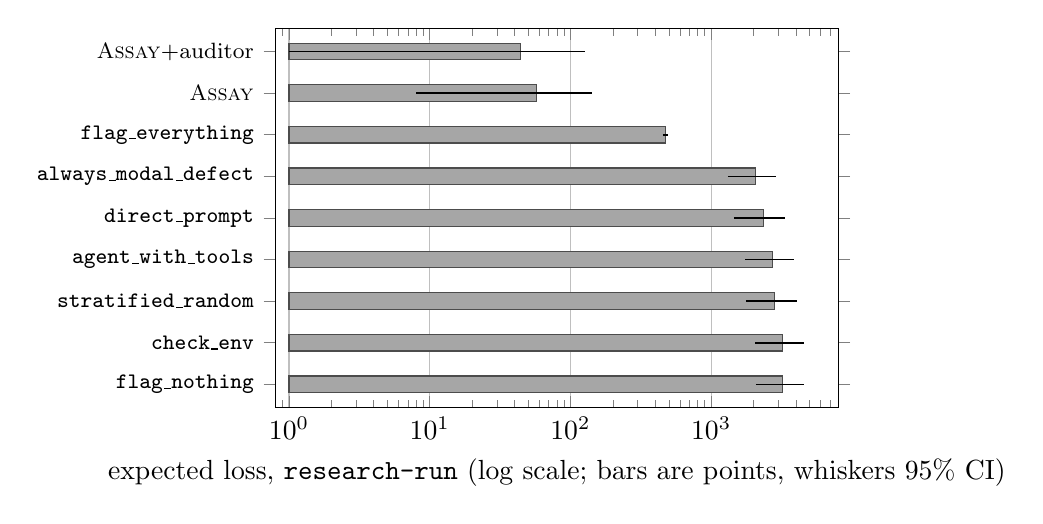
\begin{tikzpicture}
\begin{axis}[xbar, xmode=log, width=0.72\linewidth, height=6.4cm, xmin=0.8, xmax=8000,
  symbolic y coords={flagnothing,checkenv,stratifiedrandom,agentwithtools,directprompt,alwaysmodaldefect,flageverything,assay,assayplusauditor}, ytick=data, yticklabels={{\texttt{flag\_nothing}},{\texttt{check\_env}},{\texttt{stratified\_random}},{\texttt{agent\_with\_tools}},{\texttt{direct\_prompt}},{\texttt{always\_modal\_defect}},{\texttt{flag\_everything}},{\textsc{Assay}},{\textsc{Assay}+auditor}}, yticklabel style={font=\footnotesize},
  xlabel={expected loss, \texttt{research-run} (log scale; bars are points, whiskers 95\% CI)},
  bar width=6pt, xmajorgrids, enlarge y limits=0.07]
\addplot[fill=black!35, draw=black!70] coordinates {(3232.0,flagnothing) (3216.0,checkenv) (2838.0,stratifiedrandom) (2746.0,agentwithtools) (2343.0,directprompt) (2055.0,alwaysmodaldefect) (474.0,flageverything) (57.0,assay) (44.0,assayplusauditor)};
\draw[black, line width=0.6pt] (axis cs:2080.0,flagnothing) -- (axis cs:4560.0,flagnothing);
\draw[black, line width=0.6pt] (axis cs:2056.0,checkenv) -- (axis cs:4552.0,checkenv);
\draw[black, line width=0.6pt] (axis cs:1767.0,stratifiedrandom) -- (axis cs:4071.0,stratifiedrandom);
\draw[black, line width=0.6pt] (axis cs:1753.0,agentwithtools) -- (axis cs:3883.0,agentwithtools);
\draw[black, line width=0.6pt] (axis cs:1451.0,directprompt) -- (axis cs:3366.0,directprompt);
\draw[black, line width=0.6pt] (axis cs:1315.0,alwaysmodaldefect) -- (axis cs:2909.0,alwaysmodaldefect);
\draw[black, line width=0.6pt] (axis cs:453.0,flageverything) -- (axis cs:492.0,flageverything);
\draw[black, line width=0.6pt] (axis cs:8.0,assay) -- (axis cs:142.0,assay);
\draw[black, line width=0.6pt] (axis cs:1.0,assayplusauditor) -- (axis cs:126.0,assayplusauditor);
\end{axis}
\end{tikzpicture}

\caption{Expected loss by arm under \texttt{research-run} (log scale; whiskers show 95\%
environment-bootstrap intervals).}
\label{fig:arms}
\end{figure}

\paragraph{Why we lead with the restricted and prevalence-aware floors.} Figure~\ref{fig:floor}
decomposes \fe{}'s \lossFlagEverything{} false alarms. Exactly \nClassesAbsent{} of the \nClasses{}
defect classes (\texttt{EXCESSIVE\_PERMISSIONS}, \texttt{EVALUATOR\_RCE},
\texttt{DIFFICULTY\_SATURATED}, and \texttt{DIFFICULTY\_IMPOSSIBLE}) are planted in zero
environments, contributing $\nClassesAbsent{}\times\nEnv{}=\floorAbsent{}$ false alarms
(\pctFloorAbsent{}\% of \fe{}) that reflect taxonomy width rather than detection. Another
\floorClean{} false alarms (\pctFloorClean{}\%) come from \nCleanEnv{} clean environments across the
\nClassesPresent{} occurring classes, where \assay{} pays \assayCleanFA{}. Dropping the
\nClassesAbsent{} absent classes yields the restricted floor (\floorRestricted{}) and the cleaner
saving of \savedRestricted{}. Post hoc under the Bayes-optimal prevalence-aware floor (\pf{}),
\texttt{NONDETERMINISM} (MEDIUM severity, occurring in two of \nEnv{} environments, below the
threshold $1/9$) is also left unflagged on \texttt{research-run}, lowering the constant floor to
\lossPrevResearch{} (\prevFlaggedNResearch{} flagged classes). \assay{} still saves
\savedPrevResearch{} (\loSavedPrevResearch--\hiSavedPrevResearch{}, \sepPrevResearch{}); against
leave-one-out \texttt{prevalence\_floor\_loo} (\lossPrevLooResearch{}), which misses the singleton
\texttt{CONTAMINATION\_NEARDUP} defect, \assay{} saves \savedPrevLooResearch{}
(\loSavedPrevLooResearch--\hiSavedPrevLooResearch{}).

\begin{figure}[t]\centering
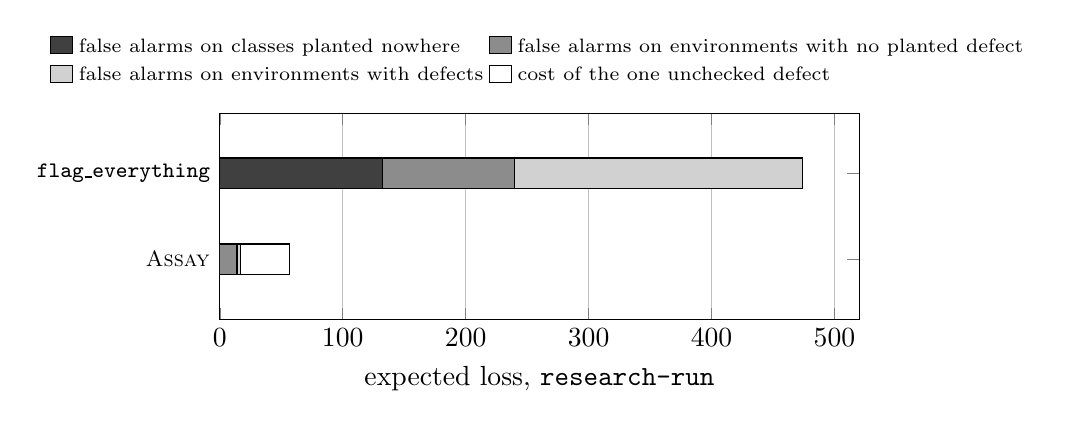
\begin{tikzpicture}
\begin{axis}[xbar stacked, width=0.8\linewidth, height=4.2cm, xmin=0, xmax=520,
  ytick={0,1}, ymin=-0.7, ymax=1.7,
  yticklabels={\textsc{Assay},\texttt{flag\_everything}}, yticklabel style={font=\footnotesize},
  xlabel={expected loss, \texttt{research-run}}, bar width=11pt, xmajorgrids,
  legend style={at={(0.5,1.08)}, anchor=south, font=\scriptsize, legend columns=2, draw=none},
  legend cell align=left]
\addplot[fill=black!75] coordinates {(132,1) (0,0)};
\addplot[fill=black!45] coordinates {(108,1) (14,0)};
\addplot[fill=black!18] coordinates {(234,1) (3,0)};
\addplot[fill=white, draw=black] coordinates {(0,1) (40,0)};
\legend{false alarms on classes planted nowhere, false alarms on environments with no planted defect, false alarms on environments with defects, cost of the one unchecked defect}
\end{axis}
\end{tikzpicture}

\caption{Decomposition of \fe{}'s loss versus \assay{}'s loss under \texttt{research-run}. Removing
the \floorAbsent{} false alarms on classes planted nowhere yields the restricted floor
(\floorRestricted{}).}
\label{fig:floor}
\end{figure}

\paragraph{All four cost profiles.} Table~\ref{tab:profiles} shows \assay{} across every cost
profile. Against unrestricted \fe{}, \assay{} separates on all four profiles (saving
\profSavedResearch{}, \profSavedProd{}, \profSavedBench{}, and \profSavedFlat{}). Against the
post hoc restricted and in-sample prevalence-aware floors, \assay{} separates on three of four
profiles (\texttt{research-run}, \texttt{benchmark-publication}, and \texttt{flat}, where \pf{}
reduces to \texttt{flag\_nothing} at \lossPrevFlat{} and \assay{} saves \savedPrevFlat{}
[\loSavedPrevFlat, \hiSavedPrevFlat]). On \texttt{production-training}, where the restricted and
prevalence-aware floors coincide at \lossRestrictedProd{}, the point saving is \savedRestrictedProd{}
but the interval crosses zero (\loSavedRestrictedProd{} to \hiSavedRestrictedProd{}): removing the
absent-class penalty reveals that separation on \texttt{production-training} rested on the
unrestricted floor. Against \texttt{prevalence\_floor\_loo} (\lossPrevLooProd{}), \assay{} separates
on all four profiles (saving \savedPrevLooProd{}, CI \loSavedPrevLooProd--\hiSavedPrevLooProd{}, on
\texttt{production-training}).

\begin{table}[t]\centering\footnotesize
\begin{tabular}{@{}lrrrrl@{}}
\toprule
profile & \textsc{Assay} & +auditor (one draw) & \texttt{flag\_everything} & saved & 95\% CI of saved \\
\midrule
\texttt{research-run} & 57.0 & 44.0 & 474.0 & 417.0 & [330, 471] \\
\texttt{production-training} & 274.0 & 248.0 & 948.0 & 674.0 & [180, 942] \\
\texttt{benchmark-publication} & 736.0 & 632.0 & 3792.0 & 3056.0 & [1800, 3768] \\
\texttt{flat} & 18.0 & 5.0 & 474.0 & 456.0 & [435, 475] \\
\bottomrule
\end{tabular}

\caption{Expected loss across all four cost profiles (\texttt{flag\_all} = \fe{}; restr. =
\fp{}; prev. = in-sample \pf{}). Columns marked $^\dagger$ are post hoc; intervals marked $^\circ$
cross zero (not separated). Against \fe{}, \assay{} separates on all four profiles.}
\label{tab:profiles}
\end{table}

\paragraph{Precision, recall, and unchecked defects.} Across the \nEnv{} environments, \assay{}
achieves recall \recAssay{} (\nTP{} of \nPlanted{} planted defects) and precision \precAssay{}
(\nSpurAssay{} spurious findings: \assayCleanFA{} on the five no-correct-answer environments and
\assayDirtyFA{} on the two $\tau^2$-bench domains). \assay{} has \missAssay{} true misses on
checkable probes (\texttt{recall\_on\_checkable} = \recChecked{}) and \nUnchecked{} unchecked defect
(\texttt{SHORTCUT\_LEAK} on \texttt{inspect\_evals/boolq}, which ships no train split so
\texttt{partial\_input\_baseline} returns \texttt{NOT\_APPLICABLE}), priced at full miss cost
(\assayMissCost{} under \texttt{research-run}).

\subsection{Sensitivity to the miss-cost constant}
\label{sec:cost}

Because \assay{}'s only priced miss is a single HIGH-severity defect priced at $C/3$, its
\texttt{research-run} loss is affine in the CRITICAL miss cost $C$: $\nSpurAssay{} + C/3$.
Unrestricted \fe{} never misses and stays constant at \lossFlagEverything{}, so the two cross at
$C = 3(\lossFlagEverything{} - \nSpurAssay{}) = \critCross{}$ (Figure~\ref{fig:cost}),
\critCrossRatio{}$\times$ the shipped anchor of \critShipped{} (a \critErrPct{}\% margin;
equivalently a HIGH miss priced at \highCross{} false alarms). Against the restricted floor
(\floorRestricted{}), the crossover is still well above the shipped anchor. Two empirical anchors
bracket $C$ without deriving it: a compute-only floor (\costGpuLo--\costGpuHi{} GPU-hours at
\$\costSpot{}/h converted at \$\costEngLo--\$\costEngHi{}/engineer-hour, giving
\costFloorLo--\costFloorHi{} engineer-hours) and a manual-repair ceiling (\costMinLo--\costMinHi{}
minutes per item over SWE-bench Verified's \costSamples{} samples, giving
\costCeilLo--\costCeilHi{} engineer-hours). On the full corpus the crossover exceeds the repair
ceiling; on the \nExternal{}-environment external split, however, \assay{} crosses \fe{} at
$C = \extCross{}$, inside the repair-effort range.

\begin{figure}[t]\centering
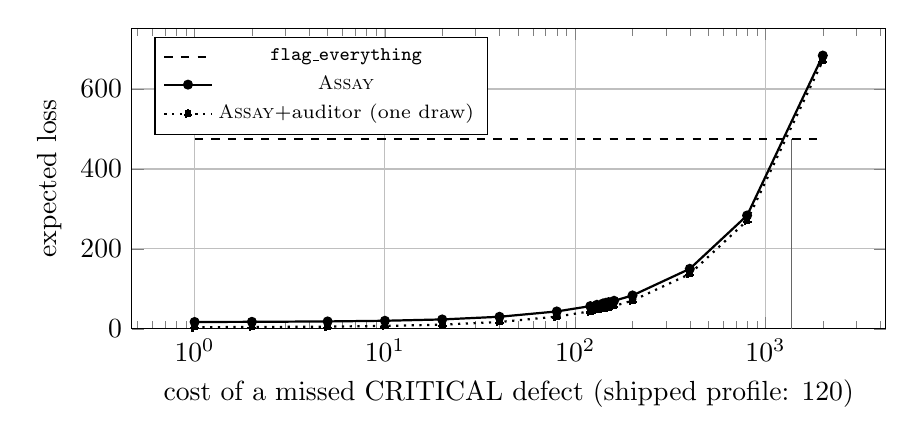
\begin{tikzpicture}
\begin{axis}[xmode=log, width=0.92\linewidth, height=5.4cm, xlabel={cost of a missed CRITICAL defect (shipped profile: 120)},
  ylabel={expected loss}, ymin=0, xmajorgrids, ymajorgrids, legend pos=north west, legend style={font=\scriptsize}]
\addplot[thick, dashed] coordinates {(1,474.0) (2,474.0) (5,474.0) (10,474.0) (20,474.0) (40,474.0) (80,474.0) (120,474.0) (130,474.0) (140,474.0) (145,474.0) (150,474.0) (160,474.0) (200,474.0) (400,474.0) (800,474.0) (2000,474.0)};
\addplot[thick, mark=*, mark size=1.4pt] coordinates {(1,17.33) (2,17.67) (5,18.67) (10,20.33) (20,23.67) (40,30.33) (80,43.67) (120,57.0) (130,60.33) (140,63.67) (145,65.33) (150,67.0) (160,70.33) (200,83.67) (400,150.33) (800,283.67) (2000,683.67)};
\addplot[thick, dotted, mark=square*, mark size=1.2pt] coordinates {(1,4.33) (2,4.67) (5,5.67) (10,7.33) (20,10.67) (40,17.33) (80,30.67) (120,44.0) (130,47.33) (140,50.67) (145,52.33) (150,54.0) (160,57.33) (200,70.67) (400,137.33) (800,270.67) (2000,670.67)};
\draw[black!60] (axis cs:1371,0) -- (axis cs:1371,474);
\legend{\texttt{flag\_everything}, \textsc{Assay}, \textsc{Assay}+auditor (one draw)}
\end{axis}
\end{tikzpicture}

\caption{Expected loss versus CRITICAL miss cost $C$ (\texttt{research-run} severity ratios held
fixed). Vertical line marks the exact crossover with \fe{} ($C=\critCross{}$).}
\label{fig:cost}
\end{figure}

\subsection{Provenance splits}
\label{sec:splits}

Splitting the corpus by authorship provenance isolates how much of the headline comes from
third-party environments (Table~\ref{tab:splits}). On the \nSelfAuthored{} self-authored
environments, \assay{} scores \selfLossAssay{} against \selfLossFloor{} for \fe{}; the
\tpfN{} third-party-format tasks score \tpfLossAssay{} against \tpfLossFloor{} after two BenchJack
exploit policies were added to the scripted Challenger during development, so neither split is
held-out evidence.

\begin{table}[t]\centering\footnotesize
\begin{tabular}{@{}lrrrrl@{}}
\toprule
split (\texttt{research-run}) & envs & planted & \textsc{Assay} & \texttt{flag\_everything} & saved [95\% CI] \\
\midrule
all published & 33 & 54 & 57.0 & 474.0 & 417.0 [330, 471] \\
self-authored & 25 & 47 & 12.0 & 353.0 & 341.0 [322, 359] \\
in-process fixtures & 15 & 19 & 12.0 & 221.0 & 209.0 [196, 221] \\
our content, third-party format & 10 & 28 & 0.0 & 132.0 & 132.0 [119, 144] \\
genuinely external & 8 & 7 & 45.0 & 121.0 & 76.0 [$-$4, 121] \emph{not separated} \\
\bottomrule
\end{tabular}

\caption{Expected loss by authorship provenance under \texttt{research-run}. The in-process split is
asserted exact by unit tests on its \nFixtures{} fixtures (its loss is the twelve false alarms on
the three authored no-answer environments).}
\label{tab:splits}
\end{table}

On the \nExternal{} genuinely external environments (\nExtPlanted{} planted defects, of which
\nPlantedExtDerived{} carry externally derived labels), \assay{} scores \extLossAssay{} against
\extLossFloor{} for \fe{}, a saving of \extSaved{} with a 95\% interval of \extLoSaved{} to
\extHiSaved{} (not separated). Precision there is \extPrec{} (\extSpur{} false alarms), recall is
\extRec{} (\extMiss{} true misses, \extUnchecked{} unchecked defect, checkable recall
\extRecChecked{}). Under \texttt{production-training} (CRITICAL cost \prodRatio{}$\times$ false
alarm), \assay{} loses to \fe{} on the external split by \extProdDelta{} (\extProdAssay{} vs.\
\extProdFloor{}, Table~\ref{tab:extprof}). Post hoc on these \nExternal{} environments under
\texttt{research-run}, only \extPrevPresentClasses{} defect classes occur, so an oracle-prior
in-sample \pf{} scores \extLossPrev{} (saving \extSavedPrev{}, CI \extLoSavedPrev{} to
\extHiSavedPrev{}), whereas leave-one-out \texttt{prevalence\_floor\_loo} scores \extLossPrevLoo{}
(saving \extSavedPrevLoo{}, CI \extLoSavedPrevLoo{} to \extHiSavedPrevLoo{}) because three of the
five classes appear in only one external environment.

\begin{table}[t]\centering\small
\begin{tabular}{@{}lrrrl@{}}
\toprule
profile (external split) & \textsc{Assay} & \texttt{flag\_everything} & saved & 95\% CI \\
\midrule
\texttt{research-run} & 45.0 & 121.0 & 76.0 & [$-$4, 121] \\
\texttt{production-training} & 250.0 & 242.0 & $-$8.0 & point only \\
\texttt{benchmark-publication} & 640.0 & 968.0 & 328.0 & point only \\
\texttt{flat} & 6.0 & 121.0 & 115.0 & point only \\
\bottomrule
\end{tabular}

\caption{Expected loss on the \nExternal{} genuinely external environments across all four cost
profiles. Bootstrap intervals are computed for \texttt{research-run}; other profiles show points.}
\label{tab:extprof}
\end{table}

\subsection{Independently confirmed defect lists}
\label{sec:external}

\paragraph{$\tau^2$-bench.} To test detection outside our own labels, we evaluated \assay{} at task
level against \tauPos{} defects confirmed by an independent team across \tauTasks{} tasks in
$\tau^2$-bench retail and airline (base rate \tauBase{}), defined mechanically as the diff between
the base and verified revisions~\citep{tau2verified}. Comparing against a random flagger issuing the
same number of flags, the full twelve-probe battery flags \tauAllFlag{} tasks and hits \tauAllTP{}
positives versus \tauAllExpTP{} expected at random (recall \tauAllRec{}, precision \tauAllPrec{},
exact one-sided $p=\tauAllP{}$): indistinguishable from chance. Excluding one advisory lexical probe
(\texttt{assert\_traceability}) leaves \tauNarFlag{} flagged tasks and \tauNarTP{} true positives
versus \tauNarExpTP{} expected (recall \tauNarRec{}, precision \tauNarPrec{}, $p=\tauNarP{}$). That
exclusion was made after inspecting the full-battery result and is uncorrected for two looks, so
$p=\tauNarP{}$ is exploratory rather than confirmatory. By upstream category (Table~\ref{tab:tau2}),
signal concentrates in verifier/annotation errors rather than evaluation ambiguity
(\tauEvalAmbDet{} of \tauEvalAmbPos{} detected), and one upstream category (\texttt{database\_accuracy},
\tauDbPos{} positives) has no corresponding class in \assay{}'s taxonomy.

\begin{table}[t]\centering\small
\begin{tabular}{@{}lrrr@{}}
\toprule
upstream category & positives & detected & recall \\
\midrule
policy compliance & 14 & 6 & 0.429 \\
database accuracy & 5 & 1 & 0.200 \\
logical consistency & 7 & 5 & 0.714 \\
evaluation ambiguity & 21 & 5 & 0.238 \\
unattributed & 15 & 4 & 0.267 \\
\bottomrule
\end{tabular}

\caption{Task-level recall on $\tau^2$-bench by upstream team category (all twelve probes).}
\label{tab:tau2}
\end{table}

\paragraph{ScienceAgentBench.} Scored with BenchGuard's own matcher against its \sabGold{} confirmed
defects, \assay{} detects \sabDetected{} and submits \sabFindings{} findings: every probe returned
\texttt{NOT\_APPLICABLE} because ScienceAgentBench is a static task set without an executable
environment or separable verifier. Taken together, the two external sets delineate \assay{}'s
structural boundary: deterministic execution probes do not detect instruction ambiguity or static
specification defects.

\subsection{The opt-in agent layer}
\label{sec:agent}

\paragraph{Language-model reader baselines.} Neither local \texttt{qwen3:8b} baseline separates from
\texttt{stratified\_random} (\lossStratRandom{}): \texttt{direct\_prompt} (\lossDirectPrompt{})
saves \savedDPvsRandom{} (\loSavedDPvsRandom{} to \hiSavedDPvsRandom{}), and
\texttt{agent\_with\_tools} (\lossAgentTools{}) scores below the random policy by
\savedRandomVsAT{} (\loSavedRandomVsAT{} to \hiSavedRandomVsAT{}). Deterministic \assay{} saves
\savedDirectPrompt{} over \texttt{direct\_prompt} and \savedAgentTools{} over
\texttt{agent\_with\_tools} (both separated).

\paragraph{Semantic gate reliability.} To address false alarms on environments without a correct
answer, \assay{}+auditor adds an opt-in language-model gate (Claude Sonnet via CLI) that may only
move scoped \texttt{DEFECT} verdicts to \texttt{NOT\_APPLICABLE}. On a standalone evaluation set
(\sgNPos{} no-answer and \sgNNeg{} graded environments at three runs each), the gate withheld false
positives in \sgTPRuns{} of \sgPosRuns{} positive runs and produced false overrides in \sgFPRuns{}
of \sgNegRuns{} negative runs (\sgFPPct{}\%). Across \gateRuns{} identical full-corpus runs
(Figure~\ref{fig:gate}; savings \gateRunValues{}), deterministic \assay{} returned \gateDetLoss{}
every time, while \assay{}+auditor saved \gateGoodMin--\gateGoodMax{} in \gateGoodRuns{} runs and
lost \gateWorstSaved{} in \gateBadRuns{} run (loss \gateWorstLoss{}), where it misclassified
\texttt{tau2/airline} as having no correct answer and suppressed two real planted defects. Because
expected loss is an expectation, the relevant summary is the mean saving of \gateMeanSaved{} rather
than the median of \gateMedianSaved{}. Three diagnostic hypotheses failed to isolate the root cause;
subsequent stress-testing of the shipped path on \texttt{tau2/airline} recorded \foFalse{} false
overrides in \foTrials{} trials (95\% upper bound \foUpper{}\%), bounding rather than explaining the
failure. Crucially, environment-level bootstrap intervals from a single draw omit this run-to-run
model variance and therefore understate uncertainty for agentic arms.

\begin{figure}[t]\centering
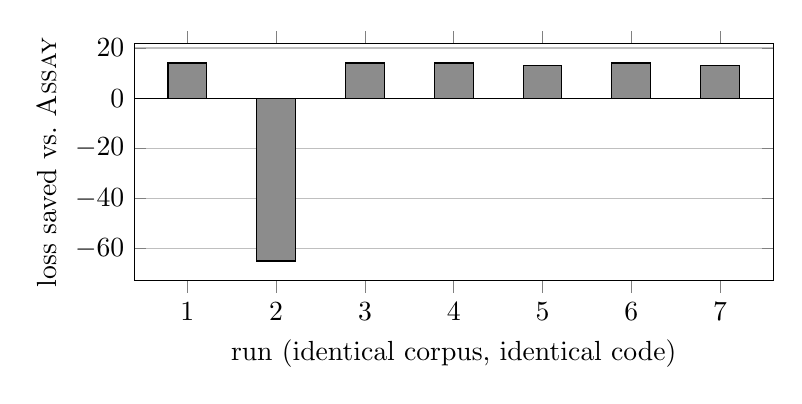
\begin{tikzpicture}
\begin{axis}[ybar, width=0.8\linewidth, height=4.6cm, xlabel={run (identical corpus, identical code)},
  ylabel={loss saved vs.\ \textsc{Assay}}, xtick={1,...,7}, ymajorgrids, bar width=14pt, enlarge x limits=0.1]
\addplot[fill=black!45] coordinates {(1,14.0) (2,-65.0) (3,14.0) (4,14.0) (5,13.0) (6,14.0) (7,13.0)};
\draw[black] (axis cs:0.4,0) -- (axis cs:7.6,0);
\end{axis}
\end{tikzpicture}

\caption{Expected-loss saving of \assay{}+auditor over deterministic \assay{} across \gateRuns{}
identical full-corpus runs. One catastrophic false override on \texttt{tau2/airline} reduces the
mean saving to \gateMeanSaved{} despite a median of \gateMedianSaved{}.}
\label{fig:gate}
\end{figure}

\paragraph{Adversarial Challenger.} In the reward-hackability probe, a prompted Claude Challenger
originally discovered an exploit class (overwriting the expected-answer file) in \ablClaudeSec{} s
where an earlier scripted attacker (\ablScriptedThenSec{} s) and \texttt{qwen3:8b} (\ablQwenSec{} s,
\ablQwenAttempts{} attempts) missed; composite reliability on that task before scripting was
\chHits{} of \chK{}. Compiling that exploit into a deterministic policy reduced runtime to
\scriptedSeconds{} s (\scriptedAttempts{} attempts) with zero model calls, leaving the prompted
agent non-load-bearing for the headline. A GRPO-trained Challenger did not close the gap, and
subsequent deduplication checks found \grpoRows{} of \grpoTotalRows{} training rows (\grpoPct{}\%)
duplicated the held-out prompt verbatim, weakening the negative result.

\section{Coverage against an external taxonomy}
\label{sec:coverage}

Mapping \assay{} onto BenchJack's eight flaw patterns (V1--V8)~\citep{wang2026benchjack} avoids
evaluating coverage solely in our own vocabulary. V5 (weak string matching) and V6 (evaluation logic
gaps) are covered broadly across adapters. V1 (isolation failure) and V7 (trusting untrusted output)
are detected for Harbor tasks via two scripted exploit policies added during development. V3 (RCE
into the evaluator) is checked statically for Python verifiers and has fired zero times on the
corpus. V8 (excessive permissions) has a probe, but no shipped third-party adapter exposes a
declared sandbox posture, so it has never executed on an external environment. V2 (answers shipped
with the test) is unimplemented, and V4 (LLM-judge prompt injection) is structurally out of scope
because \assay{} declines judge-scored verifiers. Conversely, nine of \assay{}'s \nClasses{} defect
classes have no BenchJack counterpart, and $\tau^2$-bench's \texttt{database\_accuracy} category has
no counterpart in \assay{}.

\section{Limitations}
\label{sec:limits}

\begin{itemize}\setlength\itemsep{1pt}\setlength\parskip{0pt}
\item \textbf{Corpus authorship and external sample size.} \nSelfAuthored{} of \nEnv{} environments
and \nPlantedHere{} of \nPlanted{} planted defects were authored or planted here. On the
\nExternal{} third-party environments, \assay{} does not separate from \fe{} under
\texttt{research-run} and loses under \texttt{production-training}. A blind second-rater check over
\kappaEnvs{} environments of an earlier corpus used a local \texttt{qwen3:8b} model rather than
humans and achieved \kappaAgree{}\% cell agreement ($\kappa=\kappaVal{}$), leaving labels
unconfirmed by independent human annotators.
\item \textbf{Development-set fitting and exploratory endpoints.} Probes and two scripted exploit
policies were refined on the same corpus used for scoring, with no post-freeze held-out test set.
On $\tau^2$-bench, the floor-clearing $p=\tauNarP{}$ comes from an exploratory exclusion after
seeing the chance full-battery result ($p=\tauAllP{}$) and is uncorrected for multiple looks.
\item \textbf{Floor and cost-profile dependence.} Constant floors depend on corpus class prevalence,
and removing the four absent classes eliminates bootstrap separation on
\texttt{production-training} (Table~\ref{tab:profiles}). The CRITICAL miss cost (\critShipped{}) is
a judgement rather than a derived quantity; rankings are claims about a stated cost regime.
\item \textbf{Agent variance and baseline strength.} The semantic gate's catastrophic false override
(\gateBadRuns{} of \gateRuns{} full runs) is bounded at \foUpper{}\% but unexplained, relies on a
closed model client, and is not captured by environment-level bootstrapping. The two LLM reader
baselines used a single 8B local model; a frontier reader baseline and published third-party
auditors (BenchGuard, ABA, BenchJack) were not run as comparative arms.
\item \textbf{Structural coverage.} Probes require an executable environment with a separable
verifier, placing static suites such as ScienceAgentBench and instruction-ambiguity defects out of
reach. Two real defects in shipping software (\texttt{inspect\_evals/paws} and OpenEnv's
\texttt{textarena\_env}) were verified independently and disclosed upstream; \assay{} found one and
manual inspection found the other. No claim is made about defect prevalence in the wild.
\item \textbf{Next-study scope.} Closing the external-sample, human-label, single-endpoint, and
comparator-arm gaps requires new third-party environments (thirty or more), blind human labelling
(about fifteen environments), a single pre-registered external endpoint, and paid API runs; a draft
protocol is recorded in \texttt{docs/DESIGN-V2.md} and not yet frozen or run.
\end{itemize}

\section{Conclusion}
\label{sec:conclusion}

Treating environment auditing as cost-sensitive classification forces an auditor to clear
input-ignoring floors rather than merely beat an interface linter. Across \nEnv{} environments,
\assay{}'s deterministic probe battery lowers expected loss to \lossAssay{}, saving
\savedRestricted{} over the restricted constant floor (\floorRestricted{}) and \savedPrevResearch{}
over a post hoc Bayes-optimal prevalence-aware floor (\lossPrevResearch{}), while maintaining
complete recall on checkable defects and exposing every unchecked probe explicitly.

The same evaluation framework clearly bounds what is and is not established. Savings on the
\nExternal{} genuinely external environments do not yet separate from the floor, full-battery
recall on independently labelled $\tau^2$-bench tasks is indistinguishable from random flagging due
to instruction-level defects outside execution probes' reach, and an opt-in LLM gate trades
deterministic reliability for rare catastrophic false overrides. Establishing external
generalisation requires a larger held-out third-party corpus, blind human ground truth, one
pre-registered external endpoint, and head-to-head evaluation against published benchmark auditors.

\section*{Disclosures and availability}

The code, analysis scripts, and manuscript text were written with an AI coding assistant under the
authors' direction and review. The first author works on a commercial AI gateway; nothing from that
product is used here, every component is open source or written in this repository, and all data is
public or synthetic. Code is licensed Apache-2.0 and this paper CC BY 4.0. Work on the repository
began on 2026-08-28; the first preprint version (\texttt{paper-v1.0}) was compiled and deposited on
2026-11-23, and this revision (\texttt{paper-v2.0}) is of 2026-11-23. A deposit date is not a
registration clock; pre-registrations are ordered ahead of their code in git history. This preprint
has not been peer reviewed. Code, registrations, artifacts, and table-generation scripts are at
\url{https://github.com/caiotheodoro/assay}; the corpus and Environment Cards are at
\url{https://huggingface.co/datasets/caiotheodoro/assay-corpus}; and a browser demo runs the
deterministic battery client-side at
\url{https://huggingface.co/spaces/caiotheodoro/assay-demo}.

\bibliographystyle{plainnat}
{\footnotesize\setlength{\bibsep}{1pt}\bibliography{refs}}

\appendix

\section{Pre-registrations, outcomes, and post hoc analyses}
\label{app:registrations}

All four corpus expansions that added external or no-correct-answer environments were registered in
frozen markdown documents committed before the corresponding corpus modules; the commit ordering is
verified automatically against git history by the test suite. Registrations are local repository
commits by the author rather than externally timestamped deposits. Table~\ref{tab:registrations}
summarises each registration's scope, deterministic predictions, and deviations or fired
falsification criteria.

\begin{table}[t]\centering\footnotesize
\begin{tabular}{@{}p{0.19\linewidth}p{0.20\linewidth}p{0.26\linewidth}p{0.28\linewidth}@{}}
\toprule
registration & expansion & deterministic predictions & falsification / deviations \\
\midrule
1.\ External tasks (\texttt{PRE-REGISTRATION}) & +2 external (\texttt{paws}, \texttt{boolq}; $n=24 \to 26$) & All held (\assay{} 280.0, floor 316.0, margin 36.0; \texttt{boolq} \texttt{NOT\_APPLICABLE}). & Reproducibility criterion fired: \texttt{harbor/broken-gold} flaked \texttt{NONDETERMINISM} in 1 of 6 full runs under load. \\
\addlinespace[3pt]
2.\ $\tau^2$-bench (\texttt{...-TAU2}) & +2 external ($\tau^2$ retail, airline; $n=26 \to 28$; 14$\to$16 classes) & All deterministic corpus predictions held (\assay{} 43.0, floor 394.0, 3 spurious). & One arithmetic error in external floor prediction (81.0 vs.\ 89.0); LLM vs.\ random order flipped (criterion fired). \\
\addlinespace[3pt]
3.\ No-answer set (\texttt{...-NOANSWER}) & +4 no-answer (1 external \texttt{personality\_BFI}, 3 authored; $n=28 \to 32$) & Deterministic arm held (\assay{} 56.0, floor 458.0, 16 spurious). & Gate criterion 1 fired on repeated runs (false override on \texttt{tau2/airline}); name-filter ceiling claim retracted (\#21). \\
\addlinespace[3pt]
4.\ StereoSet (\texttt{...-STEREOSET}) & +1 external no-answer (\texttt{stereoset}; $n=32 \to 33$) & All held (\assay{} 57.0, floor 474.0, 17 spurious; gate withheld \texttt{GOLD\_FAILS}). & All four criteria passed on registration run; gate later declined \texttt{stereoset} in 2 of 7 reliability runs. \\
\bottomrule
\end{tabular}

\caption{Summary of the four frozen pre-registrations, their deterministic outcomes, and every
deviation or falsification criterion that fired.}
\label{tab:registrations}
\end{table}

\paragraph{Post hoc analyses in this revision.} Two local, zero-spend additions were specified in a
pre-analysis changelog entry ahead of execution and produce no change to any pre-registered verdict:
(i) reconciling downstream \texttt{n\_missed} / \texttt{n\_unchecked} accounting in
\texttt{results/corpus\_splits.json} and \texttt{results/baselines.json} with
\texttt{results/full\_run.json} and \texttt{results/gate\_reliability.json} (fixing two loader
calls that omitted \texttt{unchecked} when rebuilding \texttt{Outcome} objects; expected loss,
recall, precision, and bootstrap intervals were unchanged, while \assay{}'s split counts moved from
one missed / zero unchecked to zero missed / one unchecked); and (ii) computing the post hoc
restricted (\fp{}) and Bayes-optimal prevalence-aware constant floors (\pf{} and
\texttt{prevalence\_floor\_loo}) across all four cost profiles in
\texttt{results/prevalence\_floor.json}.

\section{Internal red team, retractions, and repository hygiene}
\label{app:selfaudit}

During development, the repository subjected its own published documentation to an internal
red-team pass designed to falsify live claims against committed artifacts. Of \rtClaims{} claims
examined, \rtBroken{} broke, \rtPartial{} held in part, \rtWeak{} was weak, and \rtSurvives{}
survived (Table~\ref{tab:redteam}). Combined with \nRedTeamFoundAfter{} subsequent corrections
identified by external readers and automated claim checks, the repository maintains an unedited log
of \nRetractions{} retractions (\texttt{docs/RETRACTIONS.md}). Automated tests now enforce that
every number in this manuscript is generated from committed \texttt{results/*.json} files, that
downstream tables match committed bootstrap intervals, that corpus-split and reliability artifacts
agree on unchecked defects, and that CI jobs requiring optional extras skip explicitly rather than
failing silently or producing reduced-corpus headlines.

\begin{table}[t]\centering\footnotesize
\begin{tabular}{@{}rp{0.52\linewidth}p{0.34\linewidth}@{}}
\toprule
\# & claim as published & what the red team found \\
\midrule
1 & $\tau^2$-bench recall 0.339 against 62 defects & indistinguishable from random (p = 0.486) \\
2 & 24-environment corpus, assay 240.0 vs check\_env 2816.0 & half the corpus is Assay's own pytest fixtures \\
3 & ``Assay wins one of four profiles, loses two'' & flips entirely on the no-Docker corpus the README advertises \\
4 & uv run -{}-extra adapters python scripts/full\_run.py reproduces the table & that command gives 22 envs / 45 defects \\
5 & Challenger ablation table, and the ``winning policy'' snippet & matches no committed artifact \\
6 & reward\_basis was the field that needed excluding & it does not exist in either revision \\
7 & docs/REPRODUCTION.md ``expect exactly this'' & carries the retracted check\_env row \\
8 & ``a signed Environment Card'' & unkeyed digest; forgeable in three lines \\
9 & ``The incumbent is not statistically distinguishable from checking nothing'' & true by construction of the test, not by the data \\
10 & REPRODUCTION.md test counts / ``nothing skips'' & 493 passed / 18 skipped, not 275 / 0 \\
11 & SAB: ``R1 would score respectably'', ``41 findings on clean tasks'' & never scored; the file says 16 \\
12 & ``with harbor/self-graded held out so the test would mean something'' & in the README; corrected only in the changelog \\
\bottomrule
\end{tabular}

\caption{The \rtBroken{} claims broken by the internal red team, recorded verbatim as originally
published. Numbers in this table are the retracted claims, not current results.}
\label{tab:redteam}
\end{table}

\end{document}
